\section{7 Nov 23 - Activity: The Fast Fourier
Transform}\label{nov-23---activity-the-fast-fourier-transform}

We have shown how to decompose a signal using a Fourier series
decomposition:

\[V(t) = \sum_{n=-\infty}^{\infty} c_n e^{i n \omega t}\]

where we find the Fourier coefficients \(c_n\) by integrating over the
period of the signal (performing a Fourier transform of the signal):

\[c_n = \frac{1}{T} \int_0^T V(t) e^{-i n \omega t} dt\]

\subsection{Extracting the Fourier
coefficients}\label{extracting-the-fourier-coefficients}

We wrote some code earlier to perform the Fourier transform of a signal
and obtain the coefficients. We will see how to do that using the
\texttt{scipy} library later, but let's produce these results first
without it. We are going to prepare several test signals, but you will
need to make more.

\subsubsection{Test Signals}\label{test-signals}

The test signals we are going to use are:

\begin{itemize}
\tightlist
\item
  A sine wave with frequency 10 Hz and amplitude 1 V:
  \(V(t) = A\sin(2 \pi f t)\)
\item
  A sum of 3 in-phase sine waves with frequencies 10 Hz, 15 Hz, and
  30Hz, with amplitudes, 3V, 2V, and 1V respectively:
  \(V(t) = A_1 \sin(2 \pi f_1 t) + A_2 \sin(2 \pi f_2 t) + A_3 \sin(2 \pi f_3 t)\)
\item
  Both of these signals with random noise added to them.
\end{itemize}

Below we import the libraries we need and define the functions we will
use to generate the signals.

\begin{Shaded}
\begin{Highlighting}[]
\ImportTok{import}\NormalTok{ numpy }\ImportTok{as}\NormalTok{ np}
\ImportTok{import}\NormalTok{ matplotlib.pyplot }\ImportTok{as}\NormalTok{ plt}
\ImportTok{import}\NormalTok{ random}
\end{Highlighting}
\end{Shaded}

\begin{Shaded}
\begin{Highlighting}[]
\CommentTok{\# Define the functions to create signals}
\KeywordTok{def}\NormalTok{ simple\_signal(t, A}\OperatorTok{=}\DecValTok{1}\NormalTok{, f}\OperatorTok{=}\DecValTok{1}\NormalTok{):}
    \CommentTok{"""Creates a simple sinusoidal signal."""}
    \ControlFlowTok{return}\NormalTok{ A}\OperatorTok{*}\NormalTok{np.sin(}\DecValTok{2} \OperatorTok{*}\NormalTok{ np.pi }\OperatorTok{*}\NormalTok{ f}\OperatorTok{*}\NormalTok{ t)}

\KeywordTok{def}\NormalTok{ summed\_signal(t, A, f):}
    \CommentTok{"""Creates a more complex signal with multiple frequencies."""}
    \ControlFlowTok{return}\NormalTok{ A[}\DecValTok{0}\NormalTok{] }\OperatorTok{*}\NormalTok{ np.sin(}\DecValTok{2} \OperatorTok{*}\NormalTok{ np.pi }\OperatorTok{*}\NormalTok{ f[}\DecValTok{0}\NormalTok{]}\OperatorTok{*}\NormalTok{t) }\OperatorTok{+}\NormalTok{ A[}\DecValTok{1}\NormalTok{] }\OperatorTok{*}\NormalTok{ np.sin(}\DecValTok{2} \OperatorTok{*}\NormalTok{ np.pi }\OperatorTok{*}\NormalTok{ f[}\DecValTok{1}\NormalTok{]}\OperatorTok{*}\NormalTok{t}\OperatorTok{/}\NormalTok{T0) }\OperatorTok{+}\NormalTok{ A[}\DecValTok{2}\NormalTok{]}\OperatorTok{*}\NormalTok{np.sin(}\DecValTok{2} \OperatorTok{*}\NormalTok{ np.pi }\OperatorTok{*}\NormalTok{ f[}\DecValTok{2}\NormalTok{]}\OperatorTok{*}\NormalTok{t)}

\KeywordTok{def}\NormalTok{ noisy\_signal(t, A}\OperatorTok{=}\DecValTok{1}\NormalTok{, f}\OperatorTok{=}\DecValTok{1}\NormalTok{, B}\OperatorTok{=}\DecValTok{1}\NormalTok{):}
    \CommentTok{"""Creates a simple signal with random noise."""}
\NormalTok{    random.seed(}\DecValTok{42}\NormalTok{) }\CommentTok{\# seed keeps the random numbers the same each time}
\NormalTok{    noise }\OperatorTok{=}\NormalTok{ B}\OperatorTok{*}\NormalTok{np.random.normal(}\DecValTok{0}\NormalTok{, }\DecValTok{1}\NormalTok{, }\BuiltInTok{len}\NormalTok{(t)) }
    \ControlFlowTok{return}\NormalTok{ simple\_signal(t, A, f) }\OperatorTok{+}\NormalTok{ noise}

\KeywordTok{def}\NormalTok{ noisy\_summed\_signal(t, A, f, B}\OperatorTok{=}\DecValTok{1}\NormalTok{):}
    \CommentTok{"""Creates a simple signal with random noise."""}
\NormalTok{    random.seed(}\DecValTok{42}\NormalTok{) }\CommentTok{\# seed keeps the random numbers the same each time}
\NormalTok{    noise }\OperatorTok{=}\NormalTok{ B}\OperatorTok{*}\NormalTok{np.random.normal(}\DecValTok{0}\NormalTok{, }\DecValTok{1}\NormalTok{, }\BuiltInTok{len}\NormalTok{(t))}
    \ControlFlowTok{return}\NormalTok{ summed\_signal(t, A, f) }\OperatorTok{+}\NormalTok{ noise}
\end{Highlighting}
\end{Shaded}

Let's create those signals and plot them.

\begin{Shaded}
\begin{Highlighting}[]
\CommentTok{\# Set the sample rate and time}
\NormalTok{dt }\OperatorTok{=} \FloatTok{0.0005}  \CommentTok{\# Sampling frequency}
\NormalTok{T0 }\OperatorTok{=} \FloatTok{0.1} \CommentTok{\# Signal period}
\NormalTok{T }\OperatorTok{=} \FloatTok{3.0}\OperatorTok{*}\NormalTok{T0  }\CommentTok{\# Sample time length}
\NormalTok{t }\OperatorTok{=}\NormalTok{ np.arange(}\DecValTok{0}\NormalTok{, T, dt)  }\CommentTok{\# Time points}

\NormalTok{fsimple }\OperatorTok{=} \DecValTok{10}
\NormalTok{Asimple }\OperatorTok{=} \DecValTok{1}

\NormalTok{f }\OperatorTok{=}\NormalTok{ np.array([}\DecValTok{10}\NormalTok{, }\DecValTok{15}\NormalTok{, }\DecValTok{30}\NormalTok{])}
\NormalTok{A }\OperatorTok{=}\NormalTok{ np.array([}\DecValTok{3}\NormalTok{, }\DecValTok{2}\NormalTok{, }\DecValTok{1}\NormalTok{])}

\NormalTok{simple }\OperatorTok{=}\NormalTok{ simple\_signal(t, Asimple, fsimple)}
\NormalTok{summed }\OperatorTok{=}\NormalTok{ summed\_signal(t, A, f)}

\NormalTok{simple\_noise }\OperatorTok{=} \FloatTok{0.1}
\NormalTok{summed\_noise }\OperatorTok{=} \FloatTok{0.8}

\NormalTok{noisy }\OperatorTok{=}\NormalTok{ noisy\_signal(t, Asimple, fsimple, simple\_noise)}
\NormalTok{noisy\_summed }\OperatorTok{=}\NormalTok{ noisy\_summed\_signal(t, A, f, summed\_noise)}
\end{Highlighting}
\end{Shaded}

\begin{Shaded}
\begin{Highlighting}[]
\NormalTok{plt.figure(figsize}\OperatorTok{=}\NormalTok{(}\DecValTok{12}\NormalTok{, }\DecValTok{8}\NormalTok{))}
\NormalTok{plt.subplot(}\DecValTok{2}\NormalTok{, }\DecValTok{2}\NormalTok{, }\DecValTok{1}\NormalTok{)}
\NormalTok{plt.plot(t, simple)}
\NormalTok{plt.title(}\StringTok{\textquotesingle{}Simple Signal\textquotesingle{}}\NormalTok{)}
\NormalTok{plt.xlabel(}\StringTok{\textquotesingle{}Time (s)\textquotesingle{}}\NormalTok{)}
\NormalTok{plt.ylabel(}\StringTok{\textquotesingle{}Amplitude\textquotesingle{}}\NormalTok{)}

\NormalTok{plt.subplot(}\DecValTok{2}\NormalTok{, }\DecValTok{2}\NormalTok{, }\DecValTok{2}\NormalTok{)}
\NormalTok{plt.plot(t, summed)}
\NormalTok{plt.title(}\StringTok{\textquotesingle{}Summed Signal\textquotesingle{}}\NormalTok{)}
\NormalTok{plt.xlabel(}\StringTok{\textquotesingle{}Time (s)\textquotesingle{}}\NormalTok{)}
\NormalTok{plt.ylabel(}\StringTok{\textquotesingle{}Amplitude\textquotesingle{}}\NormalTok{)}

\NormalTok{plt.subplot(}\DecValTok{2}\NormalTok{, }\DecValTok{2}\NormalTok{, }\DecValTok{3}\NormalTok{)}
\NormalTok{plt.plot(t, noisy)}
\NormalTok{plt.title(}\StringTok{\textquotesingle{}Noisy Signal\textquotesingle{}}\NormalTok{)}
\NormalTok{plt.xlabel(}\StringTok{\textquotesingle{}Time (s)\textquotesingle{}}\NormalTok{)}
\NormalTok{plt.ylabel(}\StringTok{\textquotesingle{}Amplitude\textquotesingle{}}\NormalTok{)}

\NormalTok{plt.subplot(}\DecValTok{2}\NormalTok{, }\DecValTok{2}\NormalTok{, }\DecValTok{4}\NormalTok{)}
\NormalTok{plt.plot(t, noisy\_summed)}
\NormalTok{plt.title(}\StringTok{\textquotesingle{}Noisy Summed Signal\textquotesingle{}}\NormalTok{)}
\NormalTok{plt.xlabel(}\StringTok{\textquotesingle{}Time (s)\textquotesingle{}}\NormalTok{)}
\NormalTok{plt.ylabel(}\StringTok{\textquotesingle{}Amplitude\textquotesingle{}}\NormalTok{)}

\NormalTok{plt.tight\_layout()}
\end{Highlighting}
\end{Shaded}

\begin{figure}
\centering
\pandocbounded{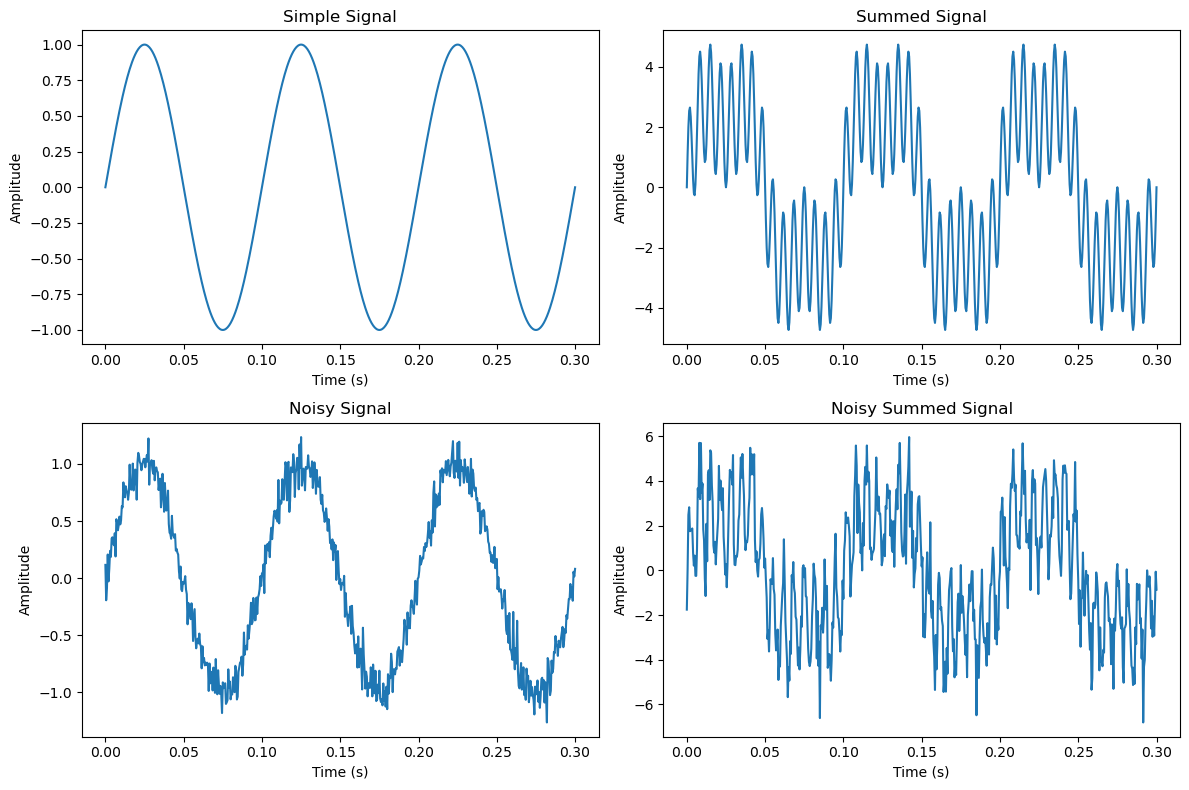
\includegraphics[keepaspectratio,alt={png}]{../images/activity-Waves-Introduction_to_FFT_activity-Waves-Introduction_to_FFT_tmp_5_0.png}}
\caption{png}
\end{figure}

\subsubsection{Find the Fourier
Components}\label{find-the-fourier-components}

\textbf{✅ Do this}

\begin{itemize}
\tightlist
\item
  Using your code from the previous activity, write a function that
  takes in a signal and returns the Fourier coefficients. You may want
  to copy and paste your code from the previous activity.
\item
  Plot the Fourier coefficients as a function of frequency. You may want
  to copy and paste your code from the previous activity.
\item
  What do you notice? Can you recover information about the original
  signal from the Fourier coefficients?
\item
  What pitfalls could you run into? Think about the Nyquist
  frequency/sampling rate.
\end{itemize}

\begin{Shaded}
\begin{Highlighting}[]
\CommentTok{\#\#\# Your code here}
\end{Highlighting}
\end{Shaded}
